% TODO fill in your paper title
\newcommand{\PaperTitle}{Simple Model Assemblages for Website Identification}
% TODO fill in your paper number when you get it
% \newcommand{\PaperNumber}{XXX}

\documentclass[10pt,sigconf,letterpaper,nonacm]{acmart}

%%%%%%%%%%%%%%%%%%%%%%%%%%%%%%%%%%%%%%%%%%%%%%%%%%%%%%%%%%%%%%%%%%%%%%%%%%%%
% This is the preamble; include packages as you see fit.
% Here are a few recommendations:
% \usepackage{color}
\usepackage{graphicx}
% \usepackage[labelformat=simple]{subcaption}
% \usepackage{xspace}
% \usepackage{multirow}
% \usepackage[ruled,vlined]{algorithm2e}
% \usepackage{ulem}
\usepackage{url}
% \normalem

%%%%%%%%%%%%%%%%%%%%%%%%%%%%%%%%%%%%%%%%%%%%%%%%%%%%%%%%%%%%%%%%%%%%%%%%%%%%

\begin{document}

\title{\PaperTitle}

\author{Charles Hu}
\email{czhu06@wm.edu}
\affiliation{
  \institution{William \& Mary}
  \city{Williamsburg}
  \state{Virginia}
  \country{USA}
}

\begin{abstract}
  In this project, we address the task of identifying the originating website given some anonymized web traffic for the purposes of gaining new insights for improving network security and optimization.
  We construct a data set of TCP streams sourced from 5 different websites: github.com, google.com, reuters.com, wikipedia.com, and youtube.com.
  With this, we develop and test 15 different machine learning models based on simple and ensemble model designs.
  We determine that a bagging ensemble model built using a decision tree provides the best performance with an accuracy score of 0.83 on the testing set, and demonstrate the capabilities of ensemble models and note the implication that web traffic data may be distinctive and generally non-overlapping.
  Challenges to this project are then analyzed and addressed with potential future avenues for improvement.
\end{abstract}

\keywords{Network trafifc, Network traffic classification, Machine learning, Ensemble models}

\maketitle

\section{Introduction}

The recent decade has witnessed a boom in use and dependency on Internet-related devices as the Internet becomes more integrated with how we live and work.
With Internet users projected to reach almost 8 billion users by 2030 \cite{forbes}, there is now a growing need for improving techniques for identifying web traffic for purposes of network security and optimization \cite{traffic} in the face of exponentially increasing web traffic both benign and malicious.
This project aims to develop a model for identifying the originating website for anonymized web traffic by observing and exploiting different patterns exhibited by different websites.

This is achieved through the development of multiple simple and ensemble models, which were trained and tested on data derived from artificial user activity across 5 different websites.
Evaluation of the models through accuracy scores on a testing set revealed that a bagging ensemble model built using a decision tree performed the best out of all developed models with a testing accuracy score of around 0.83.

Through this project, we demonstrate the feasibility of using ensemble machine learning models in improving existing techniques for network identification and management by proving their capabilities in web traffic identification.


\section{Proposed Method}

The following section details the design and rationale behind the methodology used for evaluating and classifying the website of origin for given samples of web traffic using machine learning models.

\subsection{Data Preparation}

In order to ensure that our developed models are robust and effective at their classification task, we employ a measured and systemized approach towards data collection and preprocessing to ensure that possibility of gathering ideosyncratic or erroneous data is minimized as much as possible.

The primary objective during the design of the data preparation phase was to ensure that the generated data set allows us to construct models that are effectively generalizable and not too overfit.
A key principle that allows us to achieve this is confirming that the gathered sample is as representative as possible of the general population; however, this is difficult to verify empiricaly given the complex nature of the overall population.
As a result, a preemptive approach was taken which resulted in the design of a two-stage data preparation phase comprised of a precautious data collection stage and a mitigative data preprocessing stage.
The data preparation process is summarized in Fig. ~\ref{fig:dataprep}.

\begin{figure}[h]
  \centering
  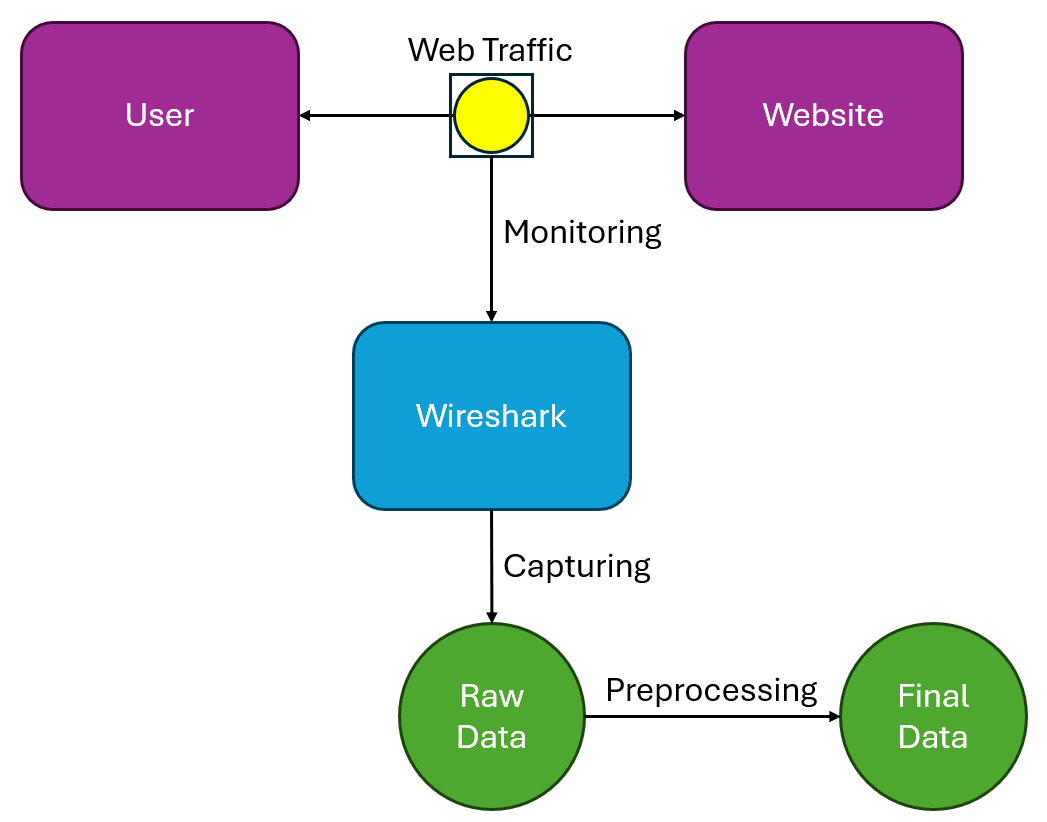
\includegraphics[width=\linewidth]{img/data_process.png}
  \caption{A diagram showing the data preparation process. It is split into 2 parts: A data collection stage and a data preprocessing stage.}
  \label{fig:dataprep}
\end{figure}

\subsubsection{Data Collection}
Data collection is performed through the monitoring of artificial website activity aimed at emulating real user interactions common to the sampled websites.
Website traffic between the user and the server hosting the website is monitored and tracked using Wireshark, an open-source software used for network traffic capture and analysis \cite{wireshark}.
Wireshark will specifically target the transport layer of network communication and intercept ongoing TCP streams between the user and the site host.
Activity on a website will occur through the controlled usage of a website's typical functionalities.
For instance, on a streaming site, the data collector will utilize the site's recommendation algorithm to view a certain number of videos before halting activity.
The goal during the activity substage is to interact with the website in a naturalistic manner akin to any typical user but avoid operations which either go beyond the scope of the target website (e.g., entering another website through an embedded link) or are unexpected of a user (e.g., manually performing HTTP operations with the website or abruptly closing the site during an interaction).
These precautions should help minimize the amount of collected TCP streams that contain information that are erroneous or overly noisy.
Once activity on a website has been concluded, Wireshark will be used to display the TCP streams generated during activity with the website (as seen in Fig. ~\ref{fig:wireshark}) and will export the TCP streams to an external CSV file for each targeted website.

\begin{figure*}[h]
  \centering
  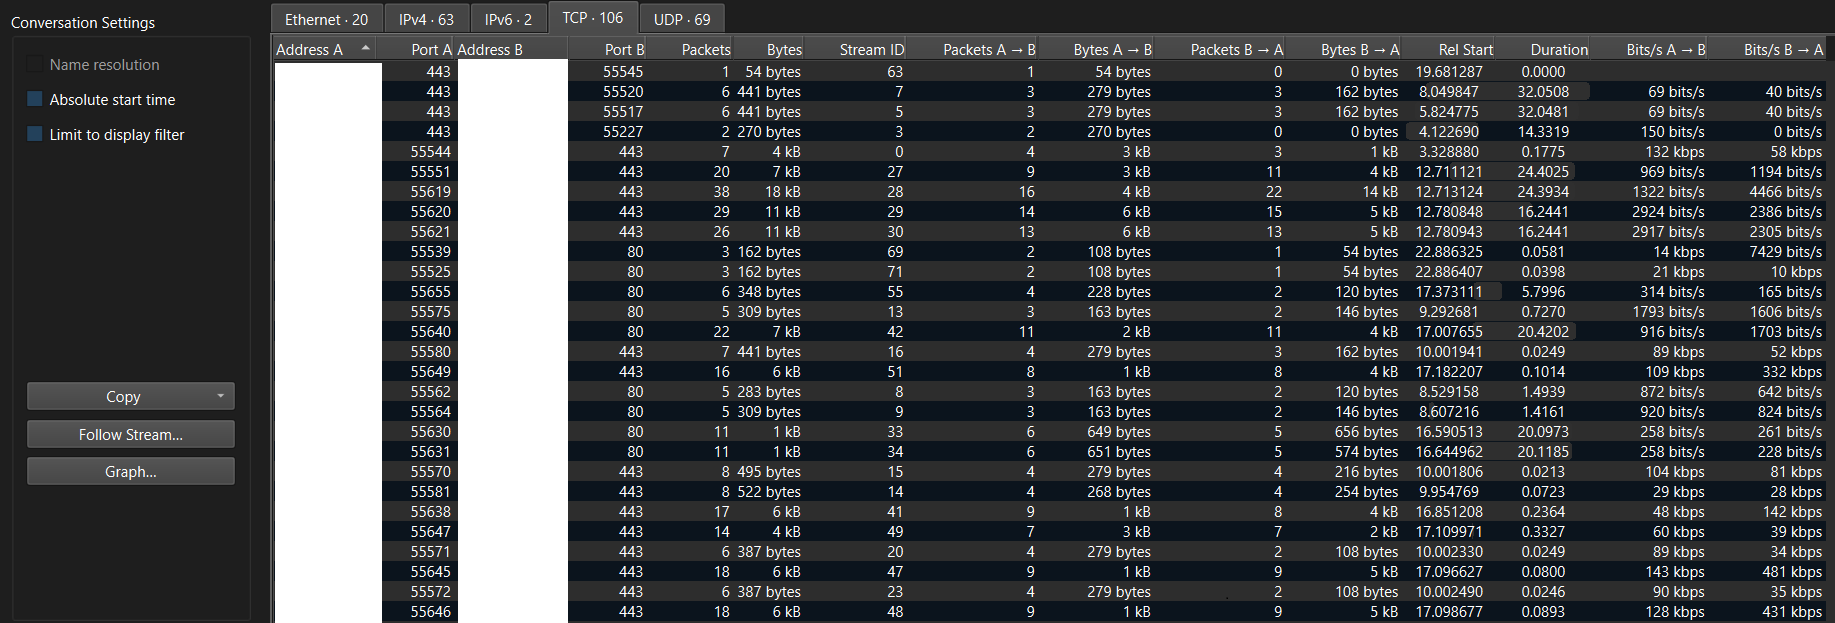
\includegraphics[width=.9\pdfpagewidth]{img/wireshark.png}
  \caption{A Wireshark window displaying tracked TCP streams and each stream's corresponding attributes. Note that IP addresses have been censored.}
  \label{fig:wireshark}
\end{figure*}

\subsubsection{Data Preprocessing}
Data preprocessing involves pruning the resulting data set from the data collection stage to remove features that are either explicitly detrimental or extraneous.
The removal of these features help improve the generalizability of our developed models by decreasing the overall model complexity and thus the variance inherent to it \cite{introInfo}; thus, if any idiosyncrasies or noise make it through our first stage of data collection, we can still reduce their influence on the overall model performance by lowering the capacity of the model to learn bad data.
To ensure that we do not develop models that have too low complexity due to a lack of learned features (and therefore trending towards too much bias in the bias-variance tradeoff), only features that are explicitly detrimental or extraneous will be removed.
Removed features are as follows:

\begin{itemize}
  \item \textbf{Address A, Port A, Address B, Port B}: These feature are explicit identifiers for the hosts in the TCP stream. Their inclusion would make the classification task redundant and would result in a model that places high importance on observing the IP and port values over other potentially useful features.
  
  \item \textbf{Stream ID}: This feature tracks the unique internal tracking ID given by Wireshark to any given TCP stream for later reference. This is Wireshark specific and not pertinent to the TCP stream itself.
  
  \item \textbf{Total Packets, Percent Filtered}: These features refer to the fitler display feature in Wireshark which filters every available packet to search for some filter specification (in this case, the target website). These are Wireshark specific and not pertinent to the TCP stream itself.
  
  \item \textbf{Rel Start}: This feature indicates when the TCP stream began relative to the start of the Wireshark network capture session. This is Wireshark specific and not pertinent to the TCP stream itself.
\end{itemize}

Retained features from the data set demonstrate either potential for aiding a model in identifying what a particular website is or are neutral in their benefit and do not actively harm or mislead the model in any way.
Retained features from the raw data set are as follows:

\begin{itemize}
  \item \textbf{Packets}: This feature tracks the total packets transferred. Note that since this is a TCP stream, this feature instead referes to a TCP segment. Different website functionalities may result in different tendencies in frequency and amount of segments transferred during a TCP stream.
  
  \item \textbf{Bytes}: This feature tracks the total amount of data in bytes that have been transferred during the entire TCP stream. Different website functionalities may result in smaller or larger sized data payloads being sent across the TCP stream.
  
  \item \textbf{Packets A $\rightarrow$ B, Bytes A $\rightarrow$ B}: These features track the packet count and total amount of data in bytes being sent from host A (the user) to host B (the site host). How intensive interactions between the user and the website are may influence these features.
  
  \item \textbf{Packets B $\rightarrow$ A, Bytes B $\rightarrow$ A}: These features track the packet count and total amount of data in bytes being sent from host B (the site host) to host A (the user). How intensive interactions between the website and the user are may influence these features.
  
  \item \textbf{Duration}: The entire time duration of the TCP stream recorded in seconds. Different durations may help indicate the purpose and level of engagement for a website.
  
  \item \textbf{Bits/s A $\rightarrow$ B, Bits/s B $\rightarrow$ A}: These features track the bitrate of the TCP stream. These features may not necessarily help the model as bitrate is subject to a number of factors that cannot be consistently attributed to a website alone, but the feature itself is not inherently detrimental so it has been left in the data set.
\end{itemize}

\subsection{Data Set}

Artificial user activity was performed and monitored across 5 websites: github.com, google.com, reuters.com, wikipedia.com, and youtube.com.
These websites were specifically chosen due to their distinct functionalities (e.g., youtube.com provides video streaming services, whereas reuters.com provides news content), which may lead to distinctive web traffic behaviors that can help in providing a direction for the trained models in the classification task.
Table ~\ref{tab:dataSize} describes the size of each class in the final data set.
TCP stream counts per website were kept roughly the same in order to prevent data set imbalance which can lead to models over prioritizing training on the larger classes.

\begin{table}[h]
  \caption{TCP stream count per website in the final cumulative data set}
  \label{tab:dataSize}
  \begin{tabular}{cc}
    \toprule
    Website & TCP Stream Count \\
    \midrule
    github & 100 \\
    google & 102 \\
    reuters & 102 \\
    wikipedia & 100 \\
    youtube & 102 \\
    \midrule
    Total & 506 \\
    \bottomrule
  \end{tabular}
\end{table}

\subsubsection{Data Analysis}

Preliminary data analysis was performed on the final data set to observe general trends and behavior.
Note that due to the small sample size of the data set, potential idiosyncrasies or noise may be exacerbated in the analysis methods.
As such, the results of these methods are only to be taken as basic guidance for handling and interpreting the data and should always be trumped by domain knowledge.
Interpretations for each analysis method will not be provided as to ensure that these methods do not influence the interpretation of the final models; however, a basic description of how they operate will be provided.
The developed models do not take these analysis results into account.

\begin{itemize}
  \item \textbf{Principal component analysis (PCA)}: A PCA was performed on the data set to observe the variability in the features (see Fig. ~\ref{fig:pca}).
  PCA is used to reduce dimensionality in a data set which can help break apart correlated data, reduce complexity, and potentially remove noise.
  A key aspect of PCA is that while dimensionality is reduced, the variability in the feature space is maintained as much as possible.
  
  \begin{figure}[t]
    \centering
    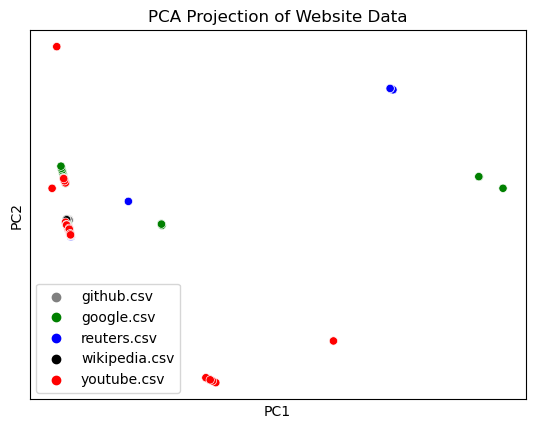
\includegraphics[width=\linewidth]{img/pca.png}
    \caption{PCA performed on the final data set.}
    \label{fig:pca}
  \end{figure}

  \item \textbf{t-distributed stochastic neighbor embedding (t-SNE)}: Like PCA, t-SNE performs dimensionality reduction but emphasizes the retention of distance-based relationships between points.
  As a result, t-SNE can sometimes help provide a low dimensional view of high dimensional relationships and groupings among points; however, distortions are likely to occur due to the inability of low dimensions to fully express the complexities of higher dimensional relationships (in a manner similar to Mercator projection maps of Earth distorting the true size of various landmasses).
  Fig. ~\ref{fig:tsne} shows a t-SNE projection performed on the final data set.

  \begin{figure}[t]
    \centering
    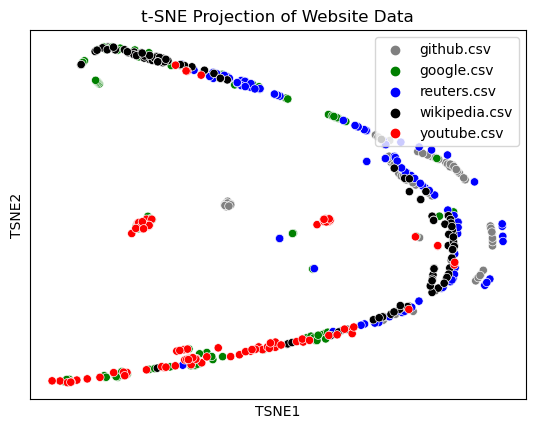
\includegraphics[width=\linewidth]{img/tsne.png}
    \caption{t-SNE performed on the final data set.}
    \label{fig:tsne}
  \end{figure}

  \item \textbf{L1 regularization}: Fig. ~\ref{fig:l1} shows L1 regularization applied to the features of the final data set.
  L1 regularization is commonly used to derive how important certain features are to the development of the final best fit model for prediction.
  The regularization is highly dependent on the specificities of the ingested data set; thus, features denoted as important should not be blindly trusted as error or noise may distort the true importance of features in the overall population.
  
  \begin{figure*}[h]
    \centering
    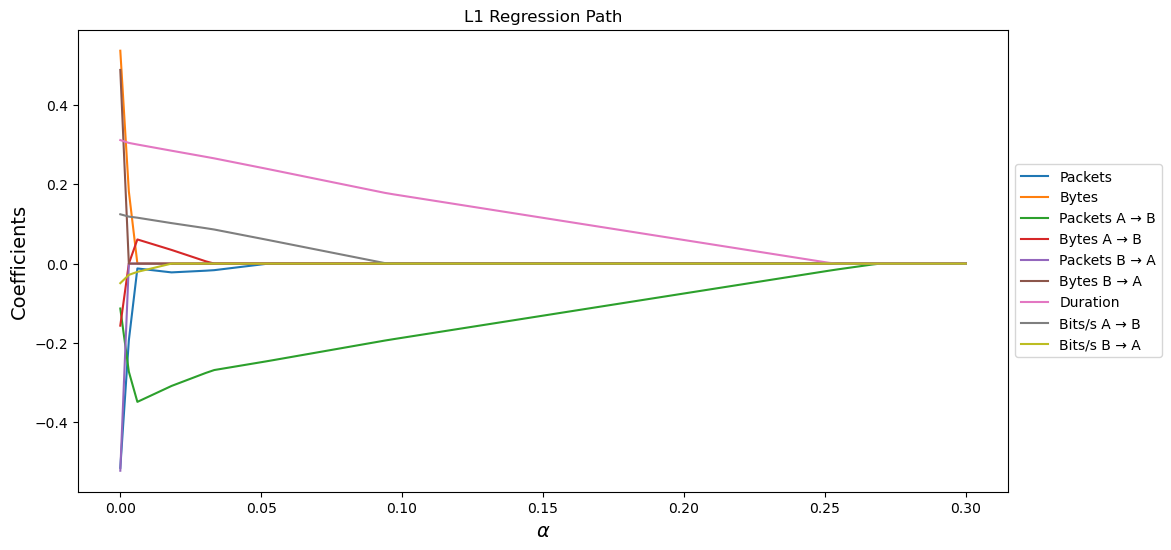
\includegraphics[width=\linewidth]{img/l1.png}
    \caption{L1 regularization performed on the final data set. The following describes the evolution of feature importance as the regularization penalty increases.}
    \label{fig:l1}
  \end{figure*}
\end{itemize}

\subsection{Model Development}

The models used for the web traffic classification task will be developed using a mix of simple models and ensemble models.
Simple models encompass basic learners (e.g., decision trees and k-nearest neighbors classifiers) which perform the classification task based on their specified learning algorithm.
Ensemble models are aggregate designs which use simple models as basic components.
They learn by varying either how its constituent component models learn and or how the results of the component models are aggregated.
A key principle to how ensemble models work is ensemble theory, which posits that a diversity of learners will result in a stronger overall learning model.
This is a result of having each constituent learner cover for its own inherent bias (i.e, weaknesses in learning certain aspects of the data set) by leveraging the strength of other constituent learners to cover for it (i.e., leverage learners which have already learned that part of the data set).
The relationship between a simple model and an ensemble model are summarized in Fig. ~\ref{fig:models}.

\begin{figure}[h]
  \centering
  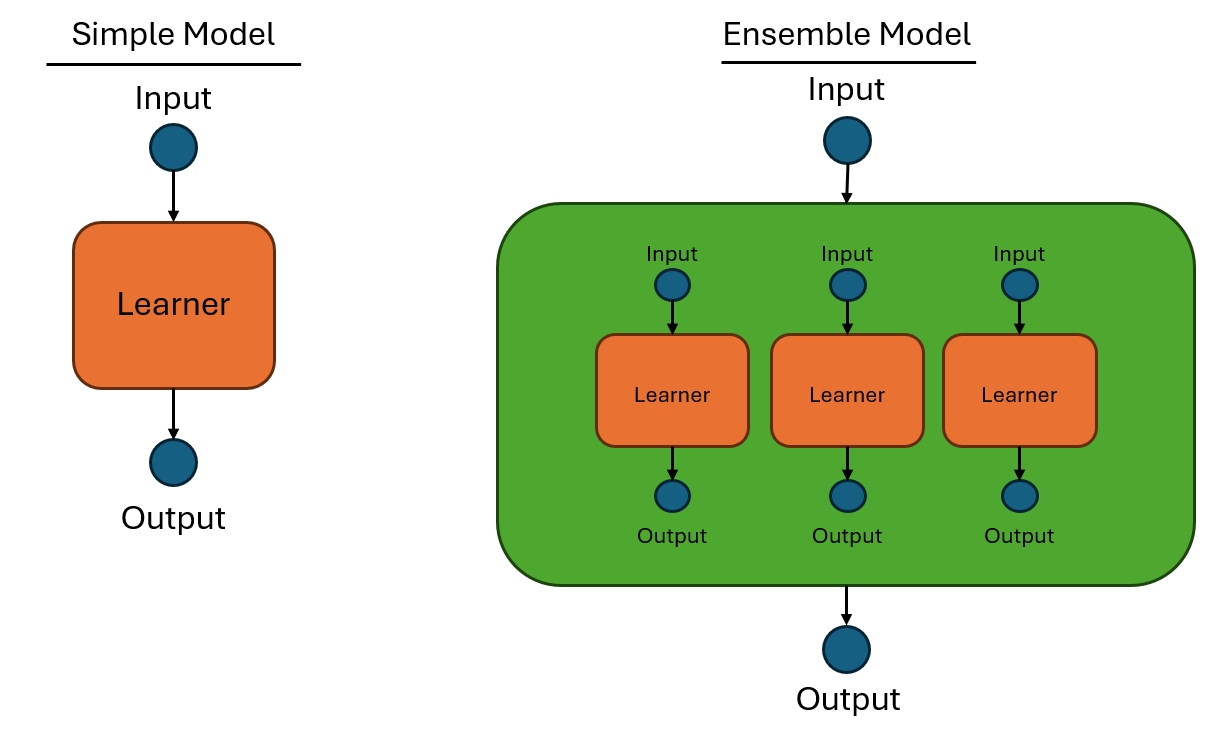
\includegraphics[width=\linewidth]{img/models.png}
  \caption{A diagram illustrating the relationship between a simple model and an ensemble model. Note that the described models are for demonstration and are not representative of the entire superset of simple and ensemble models.}
  \label{fig:models}
\end{figure}

Complex machine learning models (e.g., neural networks) will be avoided in this project due to concerns over complexity modelling capabilities.
In particular, strong complex machine learning models are more expressive in function modelling and thus are able to better capture the target function of a given data set (i.e., they are much better at learning how to replicate the data set).
This is undesirable due to our small sample size in our final data set, which means that ideosyncratic or noisy data points have less "good" (i.e., representative of the overall population) data to buffer and suppress their influence on the final model.
As a result, complex models trained on this data set have the potential to learn more bad data and generate final models which have internalized such errors and thus are no longer generalizable to our overall population.
This is mitigated by using simpler models which have less modelling capacity (i.e., more bias) and thus are less capable of modelling errors in the first place.

Developed models will be compared against a logistic regression model, which will serve as the baseline.
Models will be trained using a 8:2 training-test split ratio.
Cross-validation and hyperparameter tuning will be used when available to optimize the training of models.

\subsection{Model Specifications}

6 simple model designs and 5 ensemble model designs will be employed.
Ensemble models will be comprised of simple models that are either the best performing or most applicable.
The developed models will utilize the model implementations provided by the scikit-learn package \cite{scikit-learn}.
The details of these model designs \cite{sklearn_api, scikit_ref} are summarized in the following subsections.

\subsubsection{Simple Models}

\begin{itemize}
  \item \textbf{Decision tree classifier (DTC)}: A decision tree is an abstraction similar to a tree data structure where a model follows branching decisions driven by data which cumulatively form a tree-like structure.
  Nodes on the tree are composed of decisions which split the feature(s) and remove data from the current data set on hand based on the decision criteria.
  This typically continues until the data set on hand is only composed of a single feature (which is considered a pure node) which then becomes the leaf node of a branch.
  Classifications are based on the developed paths in the tree, where each path from the root to a leaf node corresponds to the target class which developed the path to begin with.
  
  \item \textbf{k-nearest neighbors (KNN)}: KNN operates by observing clustering and grouping within a data set. Classification occurs by attempting to find the $k$ most similar points for a given point, and classifying such point based off of the classes of those $k$ most similar points.
  The particular implementation of this design uses Euclidean distance to find the most similar points.
  
  \item \textbf{Logistic regression}: Logistic regression works by trying to find the best fit for a logistic function in the training data.
  Predictions for data are then generated using this best fit function.
  Note that though the name implies the use of regression, the implementation in scikit-learn is designed as a classifier.
  
  \item \textbf{Naive Bayes classifier}: Naive Bayes leverages Bayes' theorem to perform Bayesian probabilistic predictions of a target output given the surmised distribution of the data set.
  
  \item \textbf{Stochastic gradient descent (SGD)}: This is a specialized implementation in scikit-learn which uses stochastic gradient descent to optimize the loss function for a classifier given some input training data. 
  
  \item \textbf{Support vector classifier (SVC)}: A variation of a support vector machine designed for classification tasks. It operates by attempting to optimize the separation of different classes in the feature space using hyperplanes.
\end{itemize}

\subsubsection{Ensemble Models}

\begin{itemize}
  \item \textbf{AdaBoost}: AdaBoost takes a given weak learner and iteratively trains it using the same data set.
  It encorporates a system of internal weights where more emphasis is placed on observations which have been misclassified by the produced model.
  This results in each iteration improving at classifying observations that the preceding models were weak at.
  These new iterations are then fitted onto the original learner to produce a new strong learner.
  The AdaBoost implementation in this project is built using DTCs, logistic regression, and SGD classifiers.

  \item \textbf{Bagging}: Bagging takes a learner and trains several instances of the learner using random subsets drawn from the training data with replacement.
  The individual predictions made by these learners are then aggregated in the final ensemble model.
  The bagging implementation in this project is built using DTCs, KNNs, and logistic regression.

  \item \textbf{Random forest classifier (RFC)}: RFCs are composed of multiple decision trees built using a subset of the training data drawn with replacement.
  The aggregation in the scikit-learn implementation operates by combining the average probabilistic prediction instead of allowing each tree to vote for a final class.
  
  \item \textbf{Stacking}: Stacking takes multiple learners and stacks them on top of a final learner, where the output of each stacked learner is used as an input for the final learner to compute the final class prediction.
  The stacking implementation in this project is built using a DTC and a KNN for the stacked learners and logistic regression for the final learner.

  \item \textbf{Voting}: Voting takes several learners and trains them independently.
  It then takes the outputs of each model and counts them as votes to determine the final classification.
  The voting implementation in this project is built using a DTC, a KNN, and a logistic regression function.
  Soft (i.e., probabilistic classification) and hard (i.e., final output-based classification) voting techniques are both used.
\end{itemize}

\section{Evaluation}

The following section details the performance of the developed models on the final data set and their evaluation.

\subsection{Evaluation Metric}

The training and testing performance of the models were measured using accuracy.
Accuracy was used to provide a familiar and easily understandable metric for performance comparison.
Accuracy is specifically calculated as follows:

\begin{equation}
  \text{Accuracy} = \frac{\text{True Negative} + \text{True Positive}}{\text{Total Observations}}
\end{equation}

\subsection{Results}

The performance of the developed models was tested by having each model attempt to correctly classify the true website for a reserved testing set of TCP streams.
The following subsections describe the results of such testing.

\subsubsection{Baseline}

The performance of the logistic regression model is described in Table ~\ref{tab:log}.
Other models will be compared to this baseline to determine if they are effective at the web traffic classification task.

\begin{table}[h]
  \caption{Performance baseline for the models.}
  \label{tab:log}
  \begin{tabular}{ccc}
    \toprule
    Model & Training Accuracy & Testing Accuracy \\
    \midrule
    Log. reg. & 0.49010 & 0.55882 \\
    \bottomrule
  \end{tabular}
\end{table}

\subsubsection{Simple Model Results}

The performance of the developed simple models on the web traffic classification task are described in Table ~\ref{tab:simple}.
DTC and KNN pass the baseline with over 0.75 and 0.65 accuracy respectively, indicating that these model designs are decently capable of predicting the correct website given some unidentified TCP stream.
3 models fail to pass the baseline: SVC, SGD, and Naive Bayes.

\begin{table}[h]
  \caption{Simple model performance.}
  \label{tab:simple}
  \begin{tabular}{ccc}
    \toprule
    Model & Training Accuracy & Testing Accuracy \\
    \midrule
    DTC & 1.0 & 0.75490 \\
    KNN & 1.0 & 0.65686 \\
    SVC & 0.52475 & 0.50980 \\
    SGD & 0.42822 & 0.5 \\
    Naive Bayes & 0.39851 & 0.40196 \\
    \bottomrule
  \end{tabular}
\end{table}

\subsubsection{Ensemble Model Results}

The performance of the developed ensemble models on the web traffic classification task are described in Table ~\ref{tab:ensemble}.
Of the tested models, AdaBoost with a logistic regression function, AdaBoost with a SGD classifier, and bagging with a logistic regression function failed to pass the baseline minimum performance accuracy.
The rest of the developed models all passed the baseline minimum with bagging with a DTC, bagging with a KNN, and the RFC model performing the best across all ensemble models.
Bagging with a DTC in particular shows strong capacity to learn the data set complexity given its ability to correctly classify the testing set with about 0.83 accuracy. 

\begin{table}[h]
  \caption{Ensemble model performance.}
  \label{tab:ensemble}
  \begin{tabular}{ccc}
    \toprule
    Model & Training Accuracy & Testing Accuracy \\
    \midrule
    Bag - DTC & 0.93069 & 0.83333 \\
    Bag - KNN & 0.88366 & 0.78431 \\
    RFC & 0.97525 & 0.75490 \\
    Voting - Soft & 0.94554 & 0.75490 \\
    Ada - DTC & 0.98762 & 0.74510 \\
    Stacking & 0.95050 & 0.74510 \\
    Voting - Hard & 0.94307 & 0.72549 \\
    Ada - Log. reg. & 0.50248 & 0.50980 \\
    Ada - SGD & 0.54455 & 0.49020 \\
    Bag - Log. reg. & 0.48515 & 0.49020 \\
    \bottomrule
  \end{tabular}
\end{table}

\subsubsection{Overall Model Results}

Across both the simple models and ensemble models, bagging with a DTC performed the best with a testing accuracy of about 0.83.
All other developed models had accuracy scores below 0.80, with the closest model being bagging with a KNN with around 0.78 accuracy.
This suggests that bagging with a DTC is the most optimal model among those developed to use for confidently classifying web traffic based off of TCP streams.


\section{Discussion \& Future Work}

\subsection{Result Interpretations}

Out of 15 machine learning models developed and tested to classify web traffic, the bagging with a DTC model was the most effective and accurate classifier with about 0.83 accuracy on a reserved testing set.
Further analysis of the top performing models also reveals that 4 of the top 5 performing models were ensemble models and all of the top 5 models encorporated either a DTC or a KNN in their design.

We can first interpret these results to mean that ensemble models do generally perform better than their single model counterparts when tasked with classifying the website given some sample of web traffic.
This can be attributed to how aggregation of models works in ensemble models.
With a single model design, if the given learner is unable to learn how to properly model a part of the data set, it is always guaranteed to have poor performance accuracy whenever it encounters that part of the data set again.
With ensemble models, if one of our constituent learners is weak at learning some part of the data, we can still leverage other constituent learners in the ensemble model to learn that part of the data and cover for it.
Given that our collected TCP stream data is complex and contain mulitple features, it is expected that a simple model cannot accurately learn the data set whereas an ensemble model can.
Thus, we can interpret the superior performance of ensemble models on the web traffic classification task as reaffirming ensemble theory.

We can then interpret the dominance of DTC and KNN-based models as a sign that such models generally perform better on classifying web traffic data.
This may suggest that web traffic either clusters or is distinct and non-overlapping.
This reasoning is derived from the fact that both KNN and DTC operation on regions.
KNN operates by specifically noting spatial similarity of points and is advantageous when points of the same class tend to group together.
DTC draws decision boundaries on the data set that effectively partitions the data with each decision, effectively creating regions where it supposes classes are.
Both suggestions imply that different websites do have certain web traffic patterns which result in their TCP streams displaying distinctive traits not common to other websites; however, the former posits that this distinction is obvious whereas the latter posits that this distinction is weak.

These interpretations, if true, then contribute greatly to the problem of web traffic classification by giving us a better idea of the general patterns exhibited by the overall population of TCP stream communications.
Leveraging this would greatly help in fields such as network management and security to better improve existing techniques used for network traffic identification and management, such as optimizing traffic for in-demand web services and preventing malicious traffic intrusion \cite{traffic}.

\subsection{Future Work}

A number of challenges were encountered during this project:

\begin{itemize}
  \item \textbf{Small sample size}: The extremely limited size of the data set may result in the used sample only reflecting a small portion of the overall population.
  This would then mean that our developed models have poor generalizability due to the unrepresentative data set they were trained on.
  
  \item \textbf{Overfitting concerns}: As a result of the small sample size of the data set and the increased complexity provided by the ensemble models, there is a concern that overfitting may have occurred across the developed models. 
  
  \item \textbf{Data set concerns}: It is possible that unintended or unforeseen errors may have occurred during the data collection process.
  While the data preprocessing stage helps mitigate the effects of this, there will still be some level of influence by the bad data on the final result.
\end{itemize}

To rectify these challenges, we propose the following future work:

\begin{itemize}
  \item \textbf{Increased data set size}: Increasing the data set size used will typically also increase the representativeness of our sample on the overall population.
  Doing so would decrease the likelihood for overfitting and ensure that noise and error in the data will not be as influential on the final model.
  
  \item \textbf{Streamlined data collection process}: Streamlining and automating the data collection process will help reduce human error involved in the data collection procedure and allow more time to invest in getting more natural and representative samples of web traffic.
  
  \item \textbf{Design revision and expansion}: The interchangeable nature of learners in ensemble models opens room for potential expansion and revisiting of previously demonstrated models using new learners or hyperparameters, which can potentially reveal more about general trends in network traffic and how to capture them.
\end{itemize}


\section{Conclusion}

In this project, we aimed to develop machine learning models with the purpose of identifying which website a given sample of TCP web traffic came from.
Using a data set of TCP streams drawn from 5 different websites, we designed and trained 15 machine learning models and compared them against a logistic regression baseline.
We discovered that a bagging ensemble model built using a decision tree performed the best out of all developed models.

This project helps demonstrate a potential avenue for improving existing techniques for network identification and management by proving the capabilities of ensemble machine learning models on such a task.
We also gain the insight that web traffic, at the very least, displays distinctive generally non-overlapping behavior for websites with different functionalities.

Thus, this project serves as potential springboard for further research into using ensemble models for network traffic classification tasks which can help improve or supplement current existing techniques for web traffic identification and management.

% Note from the CFP that this section must include a statement about
% ethical issues; papers that do not include such a statement may be
% rejected.

%%%%%%%%%%%%%%%%%%%%%%%%%%%%%%%%%%%%%%%%%%%%%%%%%%%%%%%%%%%%%%%%%%%%%%%%%%%%
% We're in the endgame now

\bibliographystyle{ACM-Reference-Format}
\nocite{*}
\bibliography{refs}

\end{document}
